\section{SVBRDF Capture using MaterialGAN}
\label{sec:svbrdf:framework}

\begin{figure}[h]
	\centering
	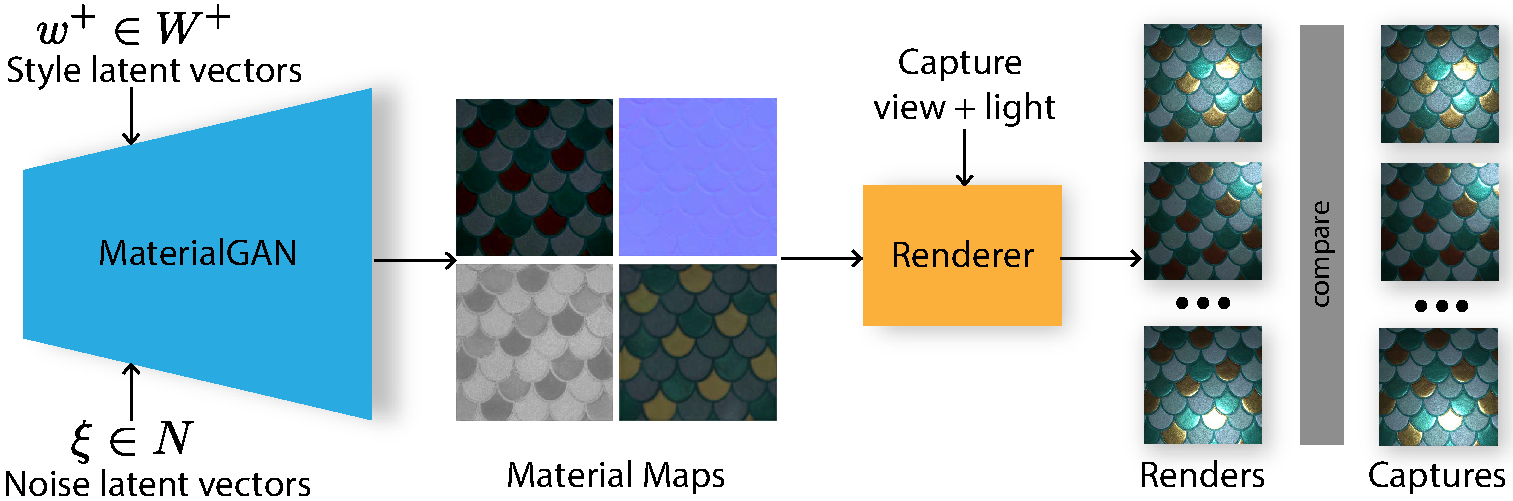
\includegraphics[width=\textwidth]{svbrdf/others/system.pdf}
	\caption[Inverse rendering pipeline]{\label{fig:svbrdf:framework}
		\textbf{Our inverse rendering pipeline.} We optimize for latent vectors $\bmw^+$ and $\bmxi$, that feed into the layers of the StyleGAN2-based MaterialGAN model. 
		The MaterialGAN generator produces material maps (diffuse albedo, normal, roughness and specular albedo), that are rendered under the captured view/light settings. 
		Finally, the renderings and measurements are compared using a combination of L2 and perceptual losses.
	}
\end{figure}


We utilize MaterialGAN, the powerful generative model described in the previous section, in a fundamentally new fashion: to \emph{capture} SVBRDF maps.
Specifically, we use MaterialGAN as a \emph{material prior} for SVBRDF acquisition via an inverse rendering framework (See Figure. \ref{fig:svbrdf:framework}).
Our goal is to estimate the SVBRDF parameter maps from one or a small number of photographs of a near-planar material sample.
We utilize a common BRDF model that involves a diffuse and a specular component using the microfacet BRDF with the GGX normal distributions \cite{walter2007microfacet}.
Our unknown parameter vectors $\bmtheta := (\bma,\bmn,r,\bms)$ encode the four per-pixel parameter maps: diffuse albedo $\bma$, surface normal $\bmn$, roughness $r$, and specular albedo $\bms$.
To recover the unknown parameter maps, we capture $k$ images $\bmI_1, \cdots, \bmI_k$.
We assume known viewing and lighting configurations for each image, which we denote as $(L_i, C_i)$.
Further, we assume that the material is lit by a single point source, collocated with the camera.
\footnote{
	In theory, non-collocated lights, area lights or projection patterns (e.g. on an LCD or similar screen) can be used as well, and would require a straightforward modification to our forward rendering process.
}
The images can be reprojected into a common frontal view (which is straightforward with a known viewing configuration).

We introduce a differentiable rendering operator $\calR$ that takes as input the parameter maps as well as the viewing and lighting configurations, and synthesizes corresponding images of the material.
Under this setup, our goal is to find values of the unknown parameters $\bmtheta$ so that renderings with these parameters match the measurements $\bmI_i$.
In other words, we focus on solving the following optimization problem:
\begin{equation}
	\label{eq:opt1}
	\bmtheta^* = \textstyle\argmin_{\bma, \bmn, r} \sum_{i=1}^k \calL(\calR(\bmtheta; \,L_i, C_i), \bmI_i),
\end{equation}
where $\calL$ is a loss function that measures the difference between the captured images, $\bmI_i$ and the renderings generated from the estimated SVBRDF parameters, $\calR(\bmtheta; \,L_i, C_i)$.


\subsection{Incorporating the MaterialGAN prior}

Eq. \eqref{eq:opt1} is, in general, a challenging optimization to solve due to its under-constrained nature.
Given a small number of input measurements, the optimization can overfit to the input, producing implausible maps that do not generalize to novel views and lighting.
To overcome this challenge, we leverage the MaterialGAN prior: instead of directly optimizing for the parameter maps $\bmtheta$,  we can optimize for a vector $\bmu$ in the MaterialGAN \emph{latent space} and map (decode) this latent vector back into material maps $\bmtheta$.
The optimization problem then becomes:
\begin{equation}
	\label{eq:opt_gan}
	\bmu^* = \textstyle\argmin_{\bmu} \sum_{i=1}^k \calL(\calR(\calG(\bmu); \,L_i, C_i), \bmI_i),
\end{equation}
where $\calG$ is the learned MaterialGAN generator.
Given that both $\calG$ and $\calR$ are differentiable operations, Eq. \eqref{eq:opt_gan} can be optimized via gradient-based methods to estimate $\bmu^*$ and the corresponding SVBRDF maps $\calG(\bmu^*)$.

The above operation is similar to recent work on embedding images in the StyleGAN latent space \cite{abdal2019image2stylegan,abdal2020image2stylegan++}.
The key difference is that we do not match material parameters directly, but evaluate their error through the rendering operator $\calR(\cdot)$.
To our knowledge, ours is the first approach to use a GAN latent space in combination with a rendering operator.


\paragraph{Loss function.}
We optimize Eq. \ref{eq:opt_gan} using a combination of a standard per-pixel L2 loss and a ``perceptual loss'' \cite{johnson2016perceptual} that has been shown to produce sharper results in image synthesis tasks:
\begin{equation}
	\label{eq:loss}
	\calL(\bmI, \bmI') = \lambda_1 \calLpix + \lambda_2 \calLper,
\end{equation}
The perceptual loss is defined as:
\begin{equation}
	\calLper(\bmI, \bmI') = \textstyle\sum_{j=1}^4 w^\mathrm{percept}_j \left\|F_j(\bmI) - F_j(\bmI')\right\|_2^2,
\end{equation}
where $F_1, \cdots, F_4$ are the flattened feature maps corresponding to the outputs of VGG-19 layers  \texttt{conv1\_1}, \texttt{conv1\_2}, \texttt{conv3\_2}, and \texttt{conv4\_2} from a pre-trained VGG network \cite{simonyan2014very}. See section \ref{ssec:optim} for more details.


\paragraph{Optimization details.}
We convert the TensorFlow-trained MaterialGAN model to PyTorch, in which our optimization framework is implemented. We optimize Eq. \ref{eq:opt_gan} using the Adam optimizer in PyTorch, with a learning rate of $0.01$. We set all other hyper-parameters to default values.
Now that our basic optimization framework is set up, there remain two key ingredients to implement our GAN-based optimization framework (Eq. \eqref{eq:opt_gan}): (i)~the choice of \emph{latent space} that we optimize $\bmu$ over, and (ii)~our optimization strategy to minimize the objective function. In the following sections, we describe our approach, along with an empirical analysis of these design choices.


\subsection{Latent space}
\label{ssec:latent}

As discussed in Sec. \ref{ssec:latent_space}, StyleGAN2 (and consequently, MaterialGAN) has a number of potential latent spaces.
In particular, MaterialGAN uses three different \emph{style} latent spaces: the input latent code $\bmz \in \calZ$ , the intermediate latent code $\bmw \in \calW$ and per-layer styles $\bmw^+ \in \calW^+$.
StyleGAN2 also injects noise $\bmxi \in \calN$ into every layer of the network to generate stochastic variations.
The typical forward generation process of the GAN only uses $\bmz$, with $\bmw$ being generated from $\bmz$ via a mapping network, and $\bmw^+$ being generated from $\bmw$ via affine transformations.
However, Abdal~et~al. \cite{abdal2019image2stylegan} note that the space of $\calZ$ is too restrictive for accurate embedding of faces or other content into the GAN space.
In other words, given the image of a human face, it is generally impossible to find a single $\bmz \in \calZ$ such that the generated image closely matches the target.
This remains the case even when extending the space to $\calW$, i.e., when searching for a $\bmw$ instead of a $\bmz$.
The space $\calW^+$, on the other hand, offers much stronger representative power.
Our experiments on embedding material maps into MaterialGAN demonstrate that optimizing for $\calW^+$ is also needed for MaterialGAN to accurately reproduce input maps.
We demonstrate this in Figure \ref{fig:svbrdf:embed}, via an experiment where we embed a given material (with known material maps) into MaterialGAN.
As shown in rows (2) and (3), maps generated by optimizing $\bmw^+ \in \calW^+$ contain more detail compared to those using $\bmw \in \calW$.

\begin{figure}[h]
	\centering
	\setlength{\resLen}{3.in}
	\setlength{\raiseLen}{0.3in}	
	\addtolength{\tabcolsep}{-3pt}
	\begin{tabular}{c @{\hspace{2\tabcolsep}} ccc}
		\raisebox{\raiseLen}{\rotatebox[origin=c]{90}{GT}} &
		\includegraphics[width=\resLen]{svbrdf/validation/embed/fake_018/tex_ref.jpg} & &
		\includegraphics[width=\resLen]{svbrdf/validation/embed/fake_037/tex_ref.jpg}
		\\
		\raisebox{\raiseLen}{\rotatebox[origin=c]{90}{$\calW$}} & 
		\includegraphics[width=\resLen]{svbrdf/validation/embed/fake_018/tex_W.jpg} & &
		\includegraphics[width=\resLen]{svbrdf/validation/embed/fake_037/tex_W.jpg}
		\\
		\raisebox{\raiseLen}{\rotatebox[origin=c]{90}{$\calW^+$}} &
		\includegraphics[width=\resLen]{svbrdf/validation/embed/fake_018/tex_W+.jpg} & &
		\includegraphics[width=\resLen]{svbrdf/validation/embed/fake_037/tex_W+.jpg}
		\\
		\raisebox{\raiseLen}{\rotatebox[origin=c]{90}{$\calW^+\calN$}} &
		\includegraphics[width=\resLen]{svbrdf/validation/embed/fake_018/tex_W+N.jpg} & &
		\includegraphics[width=\resLen]{svbrdf/validation/embed/fake_037/tex_W+N.jpg}
	\end{tabular}
	\caption[Embedding SVBRDFs into different latent spaces]{\label{fig:svbrdf:embed}
		\textbf{Embedding SVBRDFs into different latent spaces.} We take two synthetic SVBRDF material maps (top) and embed them into different latent spaces with and without the noise space (second--fourth rows). For illustration, we also embed the maps into a pure-noise space \emph{only}; this is unable to recover the color at all.
	}
\end{figure}

On the other hand, some small-scale details are still missing.
In fact, according to our experiments, only colors and large-scale features can be captured by the $\calW^+$ space.
For depicting high-frequency patterns, as demonstrated in the last row of Figure \ref{fig:svbrdf:embed}, we need to go even further and optimize the noise vector $\bmxi$ (instead of drawing it from multi-variate normal distributions).
We note that optimizing for the noise component is even more important in MaterialGAN, compared to embedding faces in StyleGAN or StyleGAN2.
We suspect that this is because with human faces, the distinction between large-scale features (e.g., eyes, noise, and mouth) and small-scale features (e.g., winkles) is very prominent, allowing the $\calW^+$ space to focus mostly on the large-scale features while leaving the small-scale ones to the noise vector $\bmxi \in \calN$.
In our case, the boundary between large-scale and small-scale material features is much less distinct.
The physical scales of real-world materials varies in a continuous fashion, making it virtually impossible to assign them to only one of the $\calW^+$ and $\calN$ spaces.
We hypothesize that for this reason, we need to focus on both $\calW^+$ and $\calN$ to achieve high-quality reconstruction of SVBRDF maps.
Based on these empirical observations, estimating SVBRDF parameter maps from photographs using our pre-trained MaterialGAN boils down to solving the following optimization:
\begin{equation}
	\bmu^* = \argmin_{\bmw^+ \in \calW^+,\, \bmxi \in \calN} \sum_{i=1}^k \calL(\calR(\calG(\bmw^+, \bmxi); \,L_i, C_i), \bmI_i).
\end{equation}
Since there are two variables $\bmw^+$ and $\bmxi$ that behave in a correlated fashion, a proper optimization strategy is crucial to achieve high-quality results. We now discuss our alternating two-step optimization method.

\subsection{Optimization strategy}
\label{ssec:optim}

Abdal et al.~\cite{abdal2019image2stylegan,abdal2020image2stylegan++} recommended using a two-stage setting by first optimizing $\bmw^+$ (with $\bmxi$ fixed) and then $\bmxi$ (with $\bmw^+$ fixed).
In our case, this approach does work in some cases but is not always the top-performing option.
In addition to this strategy, we propose two alternatives, leading to three different optimization schemes:
\begin{enumerate}
	\item \textbf{Strategy 1}: Optimize $\bmw^+$ first, then optimize $\bmxi$;
	\item \textbf{Strategy 2}: Jointly optimize both $\bmw^+$ and $\bmxi$;
	\item \textbf{Strategy 3}: Alternatively optimize $\bmw^+$ and $\bmxi$ for a small number (for example, 10) of iterations each.
\end{enumerate}

\begin{figure}[!ht]
	\centering
	\setlength{\resLen}{1.in}
	\setlength{\raiseLen}{0.4in}
	\addtolength{\tabcolsep}{-4pt}
	\begin{tabular}{cccc}
		  & SVBRDF maps & Optimization & Novel
		\\
		\raisebox{\raiseLen}{\rotatebox[origin=c]{90}{GT}} &
		\includegraphics[height=\resLen]{svbrdf/validation/optim/fake_038/ref/tex.jpg} &
		
\includegraphics[height=\resLen]{svbrdf/validation/optim/fake_038/ref/00.jpg} &
		\includegraphics[height=\resLen]{svbrdf/validation/optim/fake_038/ref/08.jpg}
		\\
		\raisebox{\raiseLen}{\rotatebox[origin=c]{0}{(1)}} &
		\includegraphics[height=\resLen]{svbrdf/validation/optim/fake_038/1000_1000/tex.jpg} &
		
\includegraphics[height=\resLen]{svbrdf/validation/optim/fake_038/1000_1000/00.jpg} &
		\includegraphics[height=\resLen]{svbrdf/validation/optim/fake_038/1000_1000/08.jpg}
		\\
		\raisebox{\raiseLen}{\rotatebox[origin=c]{0}{(2)}} &
		\includegraphics[height=\resLen]{svbrdf/validation/optim/fake_038/0_0/tex.jpg} &
		
\includegraphics[height=\resLen]{svbrdf/validation/optim/fake_038/0_0/00.jpg} &
		\includegraphics[height=\resLen]{svbrdf/validation/optim/fake_038/0_0/08.jpg}
		\\
		\raisebox{\raiseLen}{\rotatebox[origin=c]{0}{(3)}} &
		\includegraphics[height=\resLen]{svbrdf/validation/optim/fake_038/10_10/tex.jpg} &
		
\includegraphics[height=\resLen]{svbrdf/validation/optim/fake_038/10_10/00.jpg} &
		\includegraphics[height=\resLen]{svbrdf/validation/optim/fake_038/10_10/08.jpg}
	\end{tabular}
	\caption[Optimization strategy]{\label{fig:svbrdf:strategy}
		\textbf{Optimization strategy.} We evaluated three optimization strategies: (1) optimize $\bmw^+$ first, then $\bmxi$; (2) jointly optimize $\bmw^+$ and $\bmxi$; (3) alternate between $\bmw^+$ and $\bmxi$ every 10 iterations. Strategy (1) causes artifacts during the optimization, and (2) brings more noise into the maps. Particularly, for textures with small features, (1) and (2) may drive the optimization to bad local minima while the per-pixel loss could still be very low. Strategy (3) appears to be a good compromise, giving us better results in most cases. Note: ``Optimization'' means an optimized input view or its re-rendering, i.e. not a novel view.
	}
\end{figure}


Figure \ref{fig:svbrdf:strategy} shows a comparison of these strategies.
All of them give reasonable results, but Strategy 1 is better suited for materials with strong large-scale features.
Strategy 2 provides the fastest convergence because it allows the noise vector $\bmxi$ to be modified from the very beginning.
This, however, generally causes the optimization to use $\bmxi$ for encoding higher-level features and is prone to overfitting.
Finally, Strategy 3---a hybrid of Strategies 1 and 2---behaves in a more robust fashion than either of the previous strategies in most cases.
We use Strategy 3 for all the results in this chapter.
Additionally, our experiments indicate that it is desirable to use different VGG layer weights for the optimization of $\bmw^+$ and $\bmxi$. The weights we are using are, for $\bmw^+$: [1/512,1/512,1/128,1/64]; for $\bmxi$: [1/64,1/64,1/256,1/512].


\begin{figure}[!ht]
	\centering
	\setlength{\resLen}{1.in}
	\setlength{\raiseLen}{0.4in}
	\addtolength{\tabcolsep}{-4pt}
	\begin{tabular}{cccc}
		& SVBRDF maps & Optimization & Novel
		\\
		\raisebox{\raiseLen}{\rotatebox[origin=c]{90}{GT}} &
		\includegraphics[height=\resLen]{svbrdf/validation/noise_refine/fake_037/ref/tex.jpg} &
		
\includegraphics[height=\resLen]{svbrdf/validation/noise_refine/fake_037/ref/00.jpg} &
		\includegraphics[height=\resLen]{svbrdf/validation/noise_refine/fake_037/ref/07.jpg}
		\\
		\raisebox{\raiseLen}{\rotatebox[origin=c]{0}{(1)}} &
		\includegraphics[height=\resLen]{svbrdf/validation/noise_refine/fake_037/optimW+N/tex.jpg} &
		
\includegraphics[height=\resLen]{svbrdf/validation/noise_refine/fake_037/optimW+N/00.jpg} &
		\includegraphics[height=\resLen]{svbrdf/validation/noise_refine/fake_037/optimW+N/07.jpg}
		\\
		\raisebox{\raiseLen}{\rotatebox[origin=c]{0}{(2)}} &
		\includegraphics[height=\resLen]{svbrdf/validation/noise_refine/fake_037/optimW+_refine/tex.jpg} &
		
\includegraphics[height=\resLen]{svbrdf/validation/noise_refine/fake_037/optimW+_refine/00.jpg} &
		\includegraphics[height=\resLen]{svbrdf/validation/noise_refine/fake_037/optimW+_refine/07.jpg}
		\\
		\raisebox{\raiseLen}{\rotatebox[origin=c]{90}{GT}} &
		 &
		
\includegraphics[height=\resLen]{svbrdf/validation/noise_refine/real_book1/ref/00.jpg} &
		\includegraphics[height=\resLen]{svbrdf/validation/noise_refine/real_book1/ref/07.jpg}
		\\
		\raisebox{\raiseLen}{\rotatebox[origin=c]{0}{(1)}} &
		\includegraphics[height=\resLen]{svbrdf/validation/noise_refine/real_book1/optimW+N/tex.jpg} &
		
\includegraphics[height=\resLen]{svbrdf/validation/noise_refine/real_book1/optimW+N/00.jpg} &
		\includegraphics[height=\resLen]{svbrdf/validation/noise_refine/real_book1/optimW+N/07.jpg}
		\\
		\raisebox{\raiseLen}{\rotatebox[origin=c]{0}{(2)}} &
		\includegraphics[height=\resLen]{svbrdf/validation/noise_refine/real_book1/optimW+_refine/tex.jpg} &
		
\includegraphics[height=\resLen]{svbrdf/validation/noise_refine/real_book1/optimW+_refine/00.jpg} &
		\includegraphics[height=\resLen]{svbrdf/validation/noise_refine/real_book1/optimW+_refine/07.jpg}
	\end{tabular}
	\caption[Noise optimization vs. post-refinement]{\label{fig:svbrdf:noise_vs_refine}
		\textbf{Noise optimization vs. post-refinement.} (1) Optimize $\bmw^+$ and $\bmxi$ but no post-refinement; (2) Optimize $\bmw^+$ only but with post-refinement. This shows that $\bmxi$ takes an important role; optimizing only $\bmw^+$ has too little expressive power and converges to suboptimal solutions, which post-refinement cannot fix (see especially normal maps in (2)).
	}
\end{figure}

\paragraph{Noise optimization vs. post-refinement.}
\label{ssec:post-refine}
Instead of optimizing latent space $\bmw^+$ with noise $\bmxi$, another option is to apply post-refinement (that is, pixel-space optimization without any latent space) after optimizing $\bmw^+$ only. However, the space $\bmw^+$ is too small to realistically match per-pixel detail: if optimizing $\bmw^+$ only, the resulting maps have significant artifacts. Adding post-refinement to such a result essentially becomes per-pixel optimization (with little regularization), which tends to to work poorly with a small number of inputs. Optimizing $\bmxi$ offers more powerful regularization, as the noise is inserted into all layers of the generator, rather than just appended at the end (like post-refinement). We show two failure examples in Figure \ref{fig:svbrdf:noise_vs_refine}, where optimizing $\bmw^+$ leads to unsatisfactory texture maps.


\subsection{Initialization}
\label{ssec:init}

\begin{figure}[h]
	\centering
	\setlength{\resLen}{1.5in}
	\addtolength{\tabcolsep}{-4pt}
	\begin{tabular}{ll@{\hspace{8\tabcolsep}}ll}
		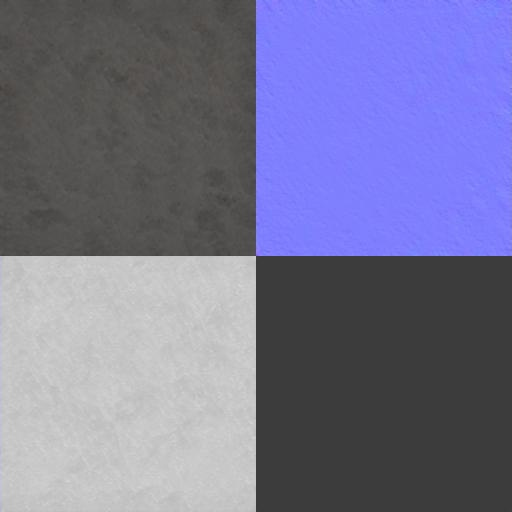
\includegraphics[width=\resLen]{svbrdf/validation/init/latent_avg_256_2x2.jpg} &
		
\includegraphics[width=\resLen]{svbrdf/validation/init/latent_avg_256_render.jpg} &
		
\includegraphics[width=\resLen]{svbrdf/validation/init/latent_const_256_2x2.jpg} &
		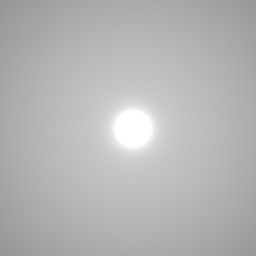
\includegraphics[width=\resLen]{svbrdf/validation/init/latent_const_256_render.jpg}
		\\
		\multicolumn{2}{c}{(a) Mean $\bmw$ initialization} & 
		\multicolumn{2}{c}{(b) Low roughness initialization} \\
	\end{tabular}
	\caption[Visualization of our constant initializations]{\label{fig:svbrdf:init}
		\textbf{Visualization of our constant initializations.} We initialize our optimization with the two materials shown here and pick the result with the lowest final loss. (This applies in cases where we do not use the result from Deschaintre et al. as initialization, as detailed in the results section and supplementary materials.) Left: Material maps generated from the mean latent vector $\bmw$. Right: An additional low roughness, specular initialization.
	}
\end{figure}

We find that our method is robust to the initialization of the latent vectors. We experimented with using the same initial configuration---represented by the material produced by the mean $\bmw$ of our GAN training data (see Figure \ref{fig:svbrdf:init}(a))---and found that is works well for most of the materials we tried (both synthetic and real).
However, this initialization represents a material with a high roughness (reflecting a bias in our training data) and sometimes leads to errors when fitting highly specular / low roughness materials.
Therefore, we add an additional low roughness initialization (see Figure \ref{fig:svbrdf:init}(b)).
In practice, given the captured images, we run our MaterialGAN optimization starting from both initializations and retain the result with the lowest optimization error of Eq. \eqref{eq:loss}.
All of our results in this chapter followed this scheme.

